\chapter{Background}
\label{chap:background}
Al fine di fornire le conoscenze necessarie alla comprensione od eventuale continuazione del lavoro svolto in questo elaborato, risulta necessario introdurre gli argomenti che si andranno ad affrontare durante la tesi, partendo dai dispositivi \textit{FPGA}.
\section{Field Programmable Gate Array}
\label{FPGA}
Sin dall'invenzione dei computer, la loro progrettazione è avvenuta con una rapida evoluzione. A metà degli anni '80, un tipo di architettura diverso da quello convenzionale fu sviluppato, le \textit{Field Programmable Gate Array} (\textit{FPGA}). Esse furono costruite tramite un'interconnessione effettuata dal progettista tra ROM/PROM o array di porte NAND.
Le \textit{FPGA} moderne sono una soluzione prefabbricata, elettronicamente programmabile, atta alla progettazione di sistemi digitali ad alte prestazioni per basso volume. Le \textit{FPGA} vengono progettate su CAD appositi, come ad esempio \textit{Vivado}, senza la necessità di dover modificare la struttura fisicamente.\clearpage
\begin{figure}[h]
\centering
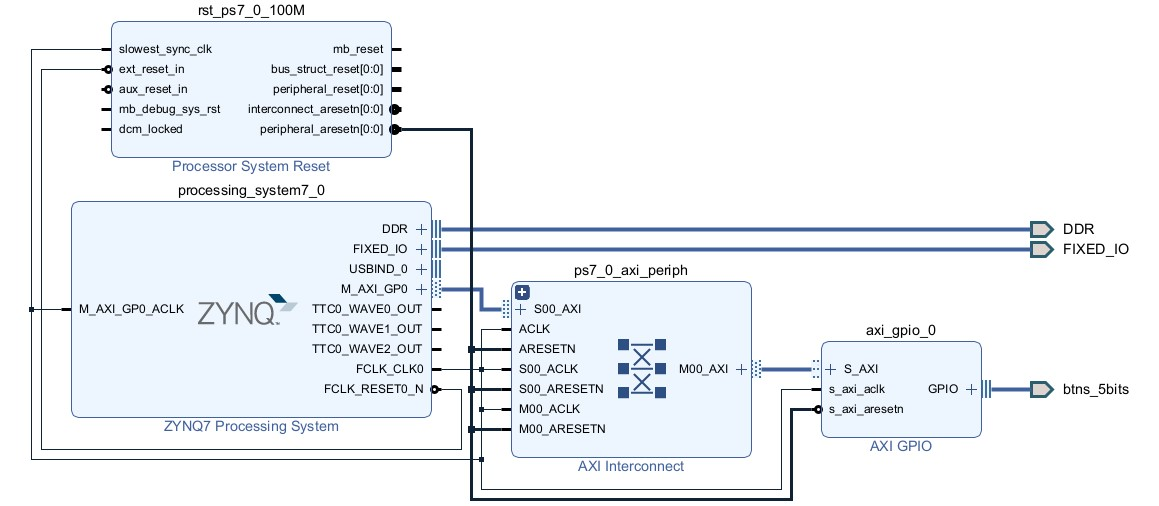
\includegraphics[width=0.8\textwidth]{images/Vivado.jpg}
\caption{Foto di una prototipazione tramite \textit{Vivado} di una \textit{FPGA Zynq-7000} che sfrutta il GPIO}
\label{VIVADO1}
\end{figure}
Questa famiglia di dispositivi dev'essere immaginata come un insieme di componenti logici; tali \textit{Configurable Logic Block} (\textit{CLB}), come già detto; possono esser modificati dal progettista. I \textit{CLB} sono composti da Look Up Table (LUT), Full Adders, Registi, Multiplexer e funzioni date dall'implementazioni.
Questa divisione in blocchi permette di creare dei cluster interconnessi, rendendo così possibile la sintetizzazione di tutte le possibili operazioni booleane e la realizzazione di sistemi complessi. 
\begin{figure}[h]
\centering
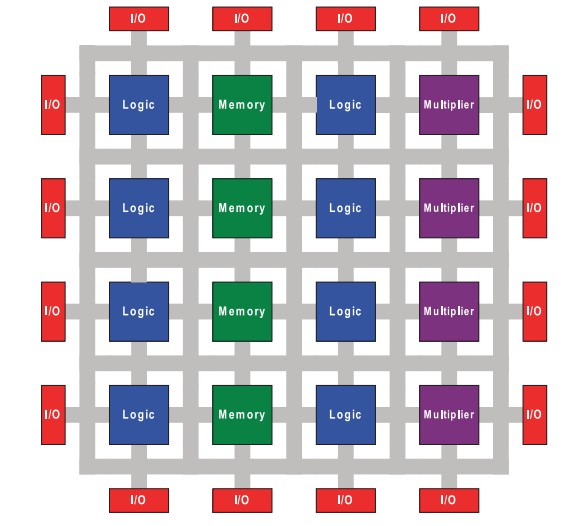
\includegraphics[width=0.3\textwidth]{images/FPGA.jpg}
\caption{Tipica rappresentazione di un \textit{FPGA} \cite{8187326}}
\end{figure}\\
Le \textit{FPGA} per loro natura devono comunicare in qualche modo con altri dispositivi: tale comunicazione è gestita da blocchi detti Input Output Block(IOB); essi garantiscono l'interfacciamento tra le risorse della \textit{Programmable Logic} (PL) ed il mondo esterno. Ogni IOB gestisce un segnale d'input/output ed è in grado di effettuare una conversione, programmabile, tra formati seriali e paralleli, oltre alla gestione di vari standard di I/O e l'eventuale configurazione di Pull-up/Pull-down interni.\\
Data la sempre più crescente quantità di CLB si può pensare come sia necessario aumentare l'area di silicio occupata, ma essa è solitamente occupata dai sistemi di interconnessione interna.\\
Le \textit{FPGA}, essendo completamente riprogrammabili, possono accogliere dei \textit{Cores} custom, detti \textit{Intellectual Property Cores}; essi rappresentano dei dispositivi pre-realizzati al fine di compiere una ben precisa azione, e possono passare da un banale moltiplicatore ad un \textit{Softcore ARM}.
\subsection{Le FPGA SoC}
L'evoluzione dei processi tecnologici ha portato alla nascita di nuovi tipi di FPGA; le\textit{ FPGA SoC}, architetture che presentano una interconnessione tra Processore, solitamente della famiglia \textit{ARM}, ed un \textit{FPGA} in un unico dispositivo.
\begin{figure}[h]
\centering
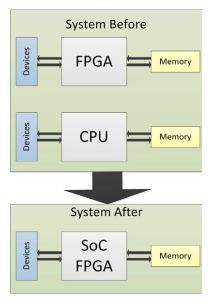
\includegraphics[width=0.35\textwidth]{images/Capture1.png}
\caption{Cambio di paradigma con l'introduzione delle FPGA SoC}
\end{figure}\\
La loro fusione permette una maggior integrazione, anche lato connettività e quindi Cloud, un minor consumo ed una comunicazione molto più efficiente tra i due grazie ad una larghezza di banda superiore ed una latenza nettamente inferiore a prima.
\begin{figure}[h]
\centering
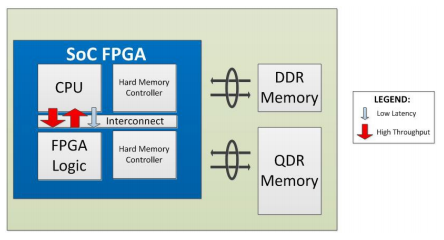
\includegraphics[width=0.5\textwidth]{images/Capture8.png}
\caption{Schema rappresentativo FPGA SoC}
\end{figure}
\subsection{Architettura Zynq-7000}
L'architettura \textit{Zynq-7000} è basata sull'architettura Xilinx All Programmable System On Chip (AP SoC). I dispositivi di questa famiglia sono formati da un dual-single Core ARM Cortex A9 su cui si basa il \textit{Processing System} (PS), includendo anche una on-chip memory, interfacce con memorie esterne e le periferiche di connettività con le interfacce, ed una \textit{Programmable Logic} (PL) a 28nm.
\begin{figure}[h]
\centering
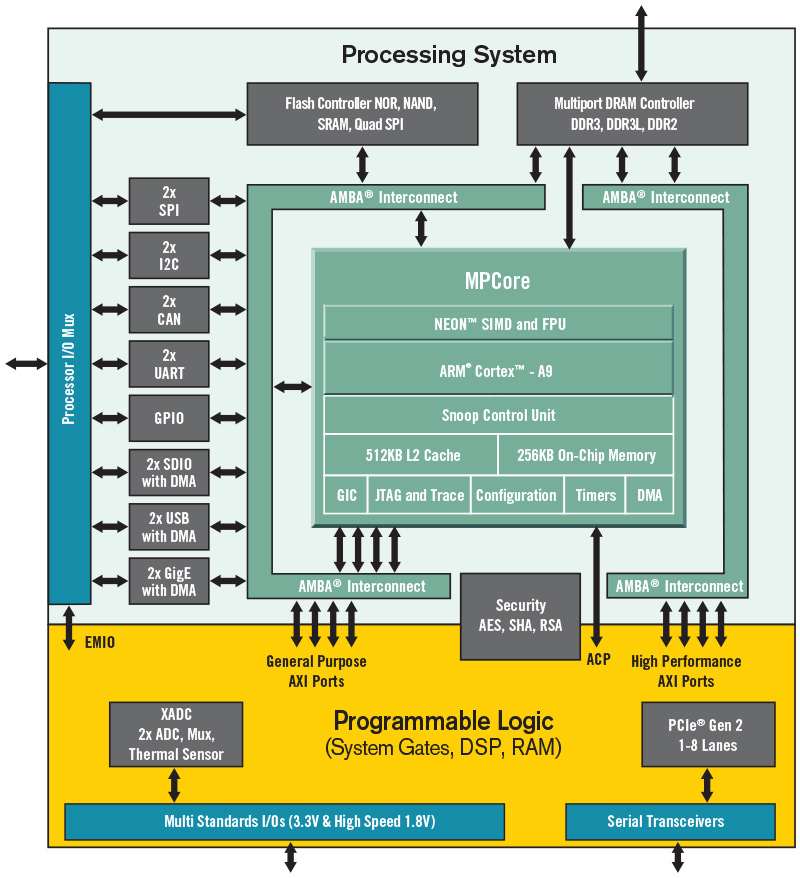
\includegraphics[width=0.4\textwidth]{images/zynq_arch.png}
\caption{Schema rappresentativo ZYNQ-7000\cite{Zynq-7000}}
\end{figure}\\
La PS e la PL sono alimentate separatamente e sarà compito del progettista decidere se disabilitare o meno la \textit{Programmable Logic}, il processore eseguirà il boot per primo e sarà sempre necessario anche per usare la parte logica, infatti si usa un approccio software centrico per la PL, ma come vedremo più avanti le due parti non sono scollegate tra di loro e questo approccio ci servirà al fine di effettuare operazioni lato PL.
\section{Linguaggi di descrizione delle FPGA}
Come accennato nel capitolo, \ref{FPGA}, le \textit{FPGA} vengono implementate tramite l'uso dei \textit{CAD} da un progettista; risulta però utile avere conoscenze dei linguaggi di descrizione dell'hardware quali \textit{VHDL}\cite{VHDL} e \textit{Verilog}\cite{Verilog} . Entrambe le opzioni sono supportate da Vivado e sono valide al fine di descrivere il comporamento di un sistema digitale. Le principali differenze tra i due linguaggi sono le similitudini al linguaggio C, infatti il Verilog ricorda molto la struttura del linguaggio di programmazione, permettendo anche ad un utente novizio la comprensione e l'approccio a questo tipo di linguaggio.\\
In generale entrambi i linguaggi sono intercambiabili per quanto rigurda la rappresentazione Register Transfer Level, ovvero la schematizzazione del sistema come un flusso di informazioni tra logica e registri. Inoltre, entrambi condividono una struttura gerarchica; è infatti  possibile tramite dei costrutti, descrivere un sistema in maniera strutturale, tramite tre possibili approcci:
\begin{itemize}
    \item Comportamentale: Il programmatore ha il compito di descrivere il comportamento di un sistema tramite un algoritmo.
    \item Strutturale: Il programmatore descrive singolarmente ogni componente interno al sistema andando poi ad usare una combinazione per rappresentare il sistema.
    \item DataFlow: Il programmatore scrive il codice emulando il flusso di dati nel sistema.
\end{itemize}
Ogni approccio necessità la presenza di un \textit{Top Level Entity}, ovvero il file principale che verrà sintetizzato e che permetterà di implementare l'\textit{FPGA}; esso conterrà tutte le componenti, codici ed eventuali librerie o supporti.
\begin{figure}[h]
\centering
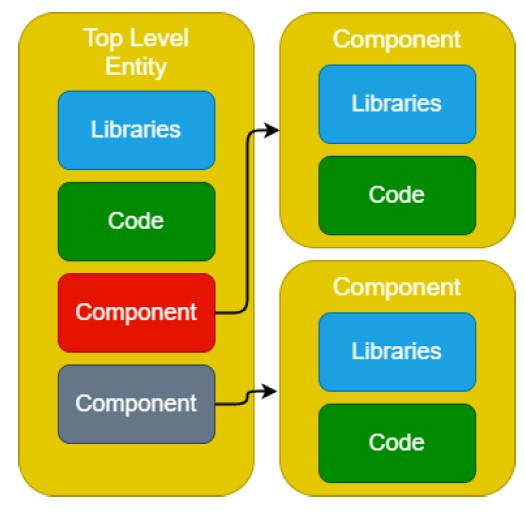
\includegraphics[width=0.3\textwidth]{images/VHFL.jpg}
\caption{Rappresentazione grafica di una Top Level Entity\cite{TesiMattia}}
\end{figure}\\
Una volta terminata la stesura del codice, bisogna specificare le specifiche e limitazioni, i \textit{constraints}, necessarie affinchè il sistema possa esser realizzato sulla scheda.
\section{Processo di Sviluppo FPGA}
Il processo di sviluppo non è riducibile alla scrittura del codice di definizione, come potrebbe avvenire per un Arduino, ma necessità dei passaggi ulteriori dovuti all'architettura, infatti la presenza dell'interconnessione dei blocchi, i blocchi I/O necessariamente configurati e la \textit{Programmable Logic} definita impongono un ulteriore livello di complessità.\\
L'evoluzione tecnologica ha comportato miglioramenti significativi per quanto riguarda lo sviluppo, infatti ad oggi si parte dalla scrittura del codice\footnote{O generazione di esso tramite vivado}, passando il tutto ad un sistema di sintesi che effettua la traduzione in una netlist, un file che descrive tutte le interconnessioni logiche da effettuare tra i vari blocchi della scheda.\\
Per capire meglio il funzionamento dividiamo il processo in tre stadi:\\
Il primo stadio, che prende il nome di \textit{Technology Mapping}, effettua la generazione di un modello \textit{RTL} (\textit{Register Transfer Level}); questo stadio converte il codice di descrizione in dei blocchi più semplici, ed è importantissimo poichè bisogna garantire che le funzionalità descritte nel codice siano rispettate; esso si verifica tramite delle simulazioni. Alcuni blocchi di logica complessa vengono portati ad un livello composto tra gate logici e registri: questo livello è detto Logic Gate Level.
\begin{figure}[h]
\centering
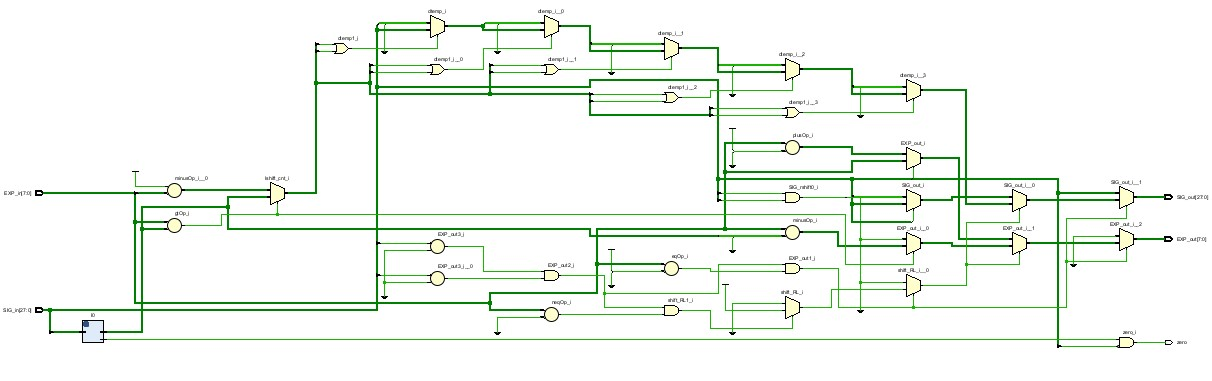
\includegraphics[width=0.8\textwidth]{images/RTL.jpg}
\caption{Rappresentazione grafica del Tecnology Mapping del FPGA in figura \ref{VIVADO1}}
\end{figure}\clearpage
Tutto questo processo viene ottimizzato come farebbe un compilatore, al fine di occupare meno spazio.\\
Una volta completato questo passaggio bisogna effettuare la collocazione degli elementi dell'FPGA: il procedimento prende il nome di \textit{Place \& Route} (\textit{PnR}), ed è a sua volta composto da tre sotto passaggi.\\
Il primo è il \textit{Packing}, che analizza le primitive e le organizza in un cluster.\\
Il secondo è il \textit{Placing}, che prende in ingresso i cluster e decide dove collocare fisicamente i componenti sulla scheda permettendo cosi l'instradamento
\begin{figure}[h]
\centering
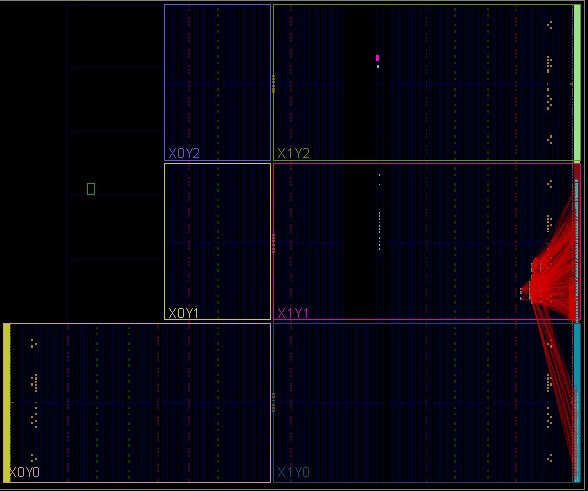
\includegraphics[width=0.4\textwidth]{images/Place.jpg}
\caption{Rappresentazione grafica del Placing del FPGA in figura \ref{VIVADO1}}
\end{figure}\\
Infine il \textit{Routing}, si occuperà di calcolare tutte le possibili connessioni selezionando la migliore, in funzione del ritardo: questo, ovviamente, rende il passaggio oneroso computazionalmente.
\begin{figure}[h]
\centering
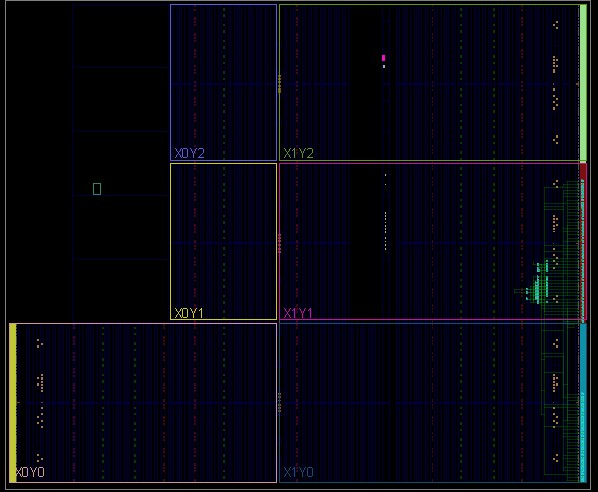
\includegraphics[width=0.4\textwidth]{images/Route.jpg}
\caption{Rappresentazione grafica del Routing del FPGA in figura \ref{VIVADO1}}
\end{figure}\\
Una volta terminati questi passaggi avremo a disposizione l'implementazione del \textit{FPGA}, ma sarà necessario tradurre il tutto in un formato interpretabile al dispositivo; questo processo verrà ripreso anche in seguito. Questo passaggio di traduzione prende il nome di generazione del bitstream.
\begin{figure}[h]
\centering
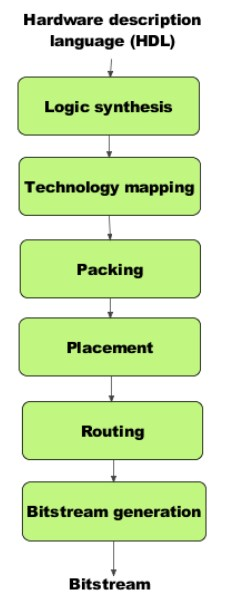
\includegraphics[width=0.2\textwidth]{images/Stack.jpg}
\caption{Stack per lo sviluppo di un FPGA}
\end{figure}\\
Questo tipo di sviluppo è il migliore nel nostro caso, poichè non stiamo effettuando un \textit{High Level Synthesis} (\textit{HLS}), in quel caso esistono dei tools appositi.
\subsection{Sviluppo tramite Vivado}
Lo sviluppo tramite \textit{Vivado} è alquanto semplificato, poichè godendo di un'interfaccia grafica permette l'implementazione di sistemi complessi anche non avendo alcuna conoscenza di \textit{VHDL} o \textit{Verilog}; si rimanda, però, all'appendice \ref{app:a} per maggiori chiarimenti su installazione ed inizio del primo progetto.
\section{Tecnologie implementative}
\subsection{Vitis}
\textit{Vitis} è il \textit{Software Development Kit} (\textit{SDK}) fornito da Xilnix nella sua suite di prodotti la sua installazione è contestuale a quella trattata in \ref{app:a}, e tramite esso è possibile generare codice  in grado di esser eseguito sulla scheda. Questo è possibile per mezzo delle le informazioni sulla scheda implementata tramite \textit{Vivado}.\\
Sono presenti due possibilità di programmazione: \textit{Standalone} e \textit{Linux}. La prima applicazione permetterà l'esecuzione di codice C in modalità \textit{Bare-Metal}\footnote{Livello di programmazione senza astrazioni, come il sistema operativo}; in questo modo potremo usare delle librerie della Xilinix che contengono delle funzioni standard al fine di effettuare la comunicazione tra PS e PL. Successivamente tratteremo anche la comunicazione tra PS e PL su sistema Linux. Questo tipo di programmazione è discussa approfonditamente \ref{Standalone}
\subsection{Petalinux}
È un tool della Xilnix necessario qualora si volesse usare una distro Linux embedded su di una \textit{FPGA SoC} Xilnix; la sua installazione è trattata in \ref{petalinuxinst}. \textit{Petalinux} offre una grossa flessibilità per la costruzione e compilazione di un kernel Linux, la sua flessibilità ci permette di escludere o includere moduli pre-esistenti, oppure di crearne uno a seconda delle esigenze. Si basa fortemente sull'architettura e sull'esportazione che avviene da \textit{Vivado} al fine di costruire il device tree e gli strumenti necessari al kernel.\\
Al fine di usufruire di \textit{Petalinux} si rende necessario impostare i Jumpers della scheda \textit{MIO2-6} in configurazione  "00110": in questo modo potremo usare il kernel creato e compilato\footnote{Verrà trattato successivamente}, tramite la scheda SD che dovrà rispettare delle specifiche espresse in \ref{sd}.
\subsection{Bootgen}
\textit{Bootgen} è un tool appartenente alla suite di sviluppo della Xilnix, il suo scopo è quello di generare i file binari e tutti gli artefatti necessari. La sua installazione verrà discussa in \ref{installazioneBoot}
Sfortunatamente questo tool è attualmente disponibile solo per architettura x86, per cui come tutti i tool presentati precedentemente, non sarà possibile installarlo sulla piattaforma da noi prescelta.\clearpage
\subsection{OpenStack}
\textit{OpenStack} è un piattaforma Cloud open-source\cite{OpenStack2} che permette la gestione di risorse in Cloud. Le risorse possono variare: da macchine virtuali a blocchi d'indirizzamento, spazio d'archiviazione ed acceleratori. Tutte le risorse fisiche vengono aggregate in un unico grande pool ed alloca le risorse virtuali, permettendo così la richiesta tramite le API da parte dell'utente finale, \textit{OpenStack} non gestisce la virtualizzazione, ma sfrutta le tecnologie di virtualizzazioni preesistenti, eseguendo un funzionamento assimilabile a quello di un raccoglitore.
\begin{figure}[h]
\centering
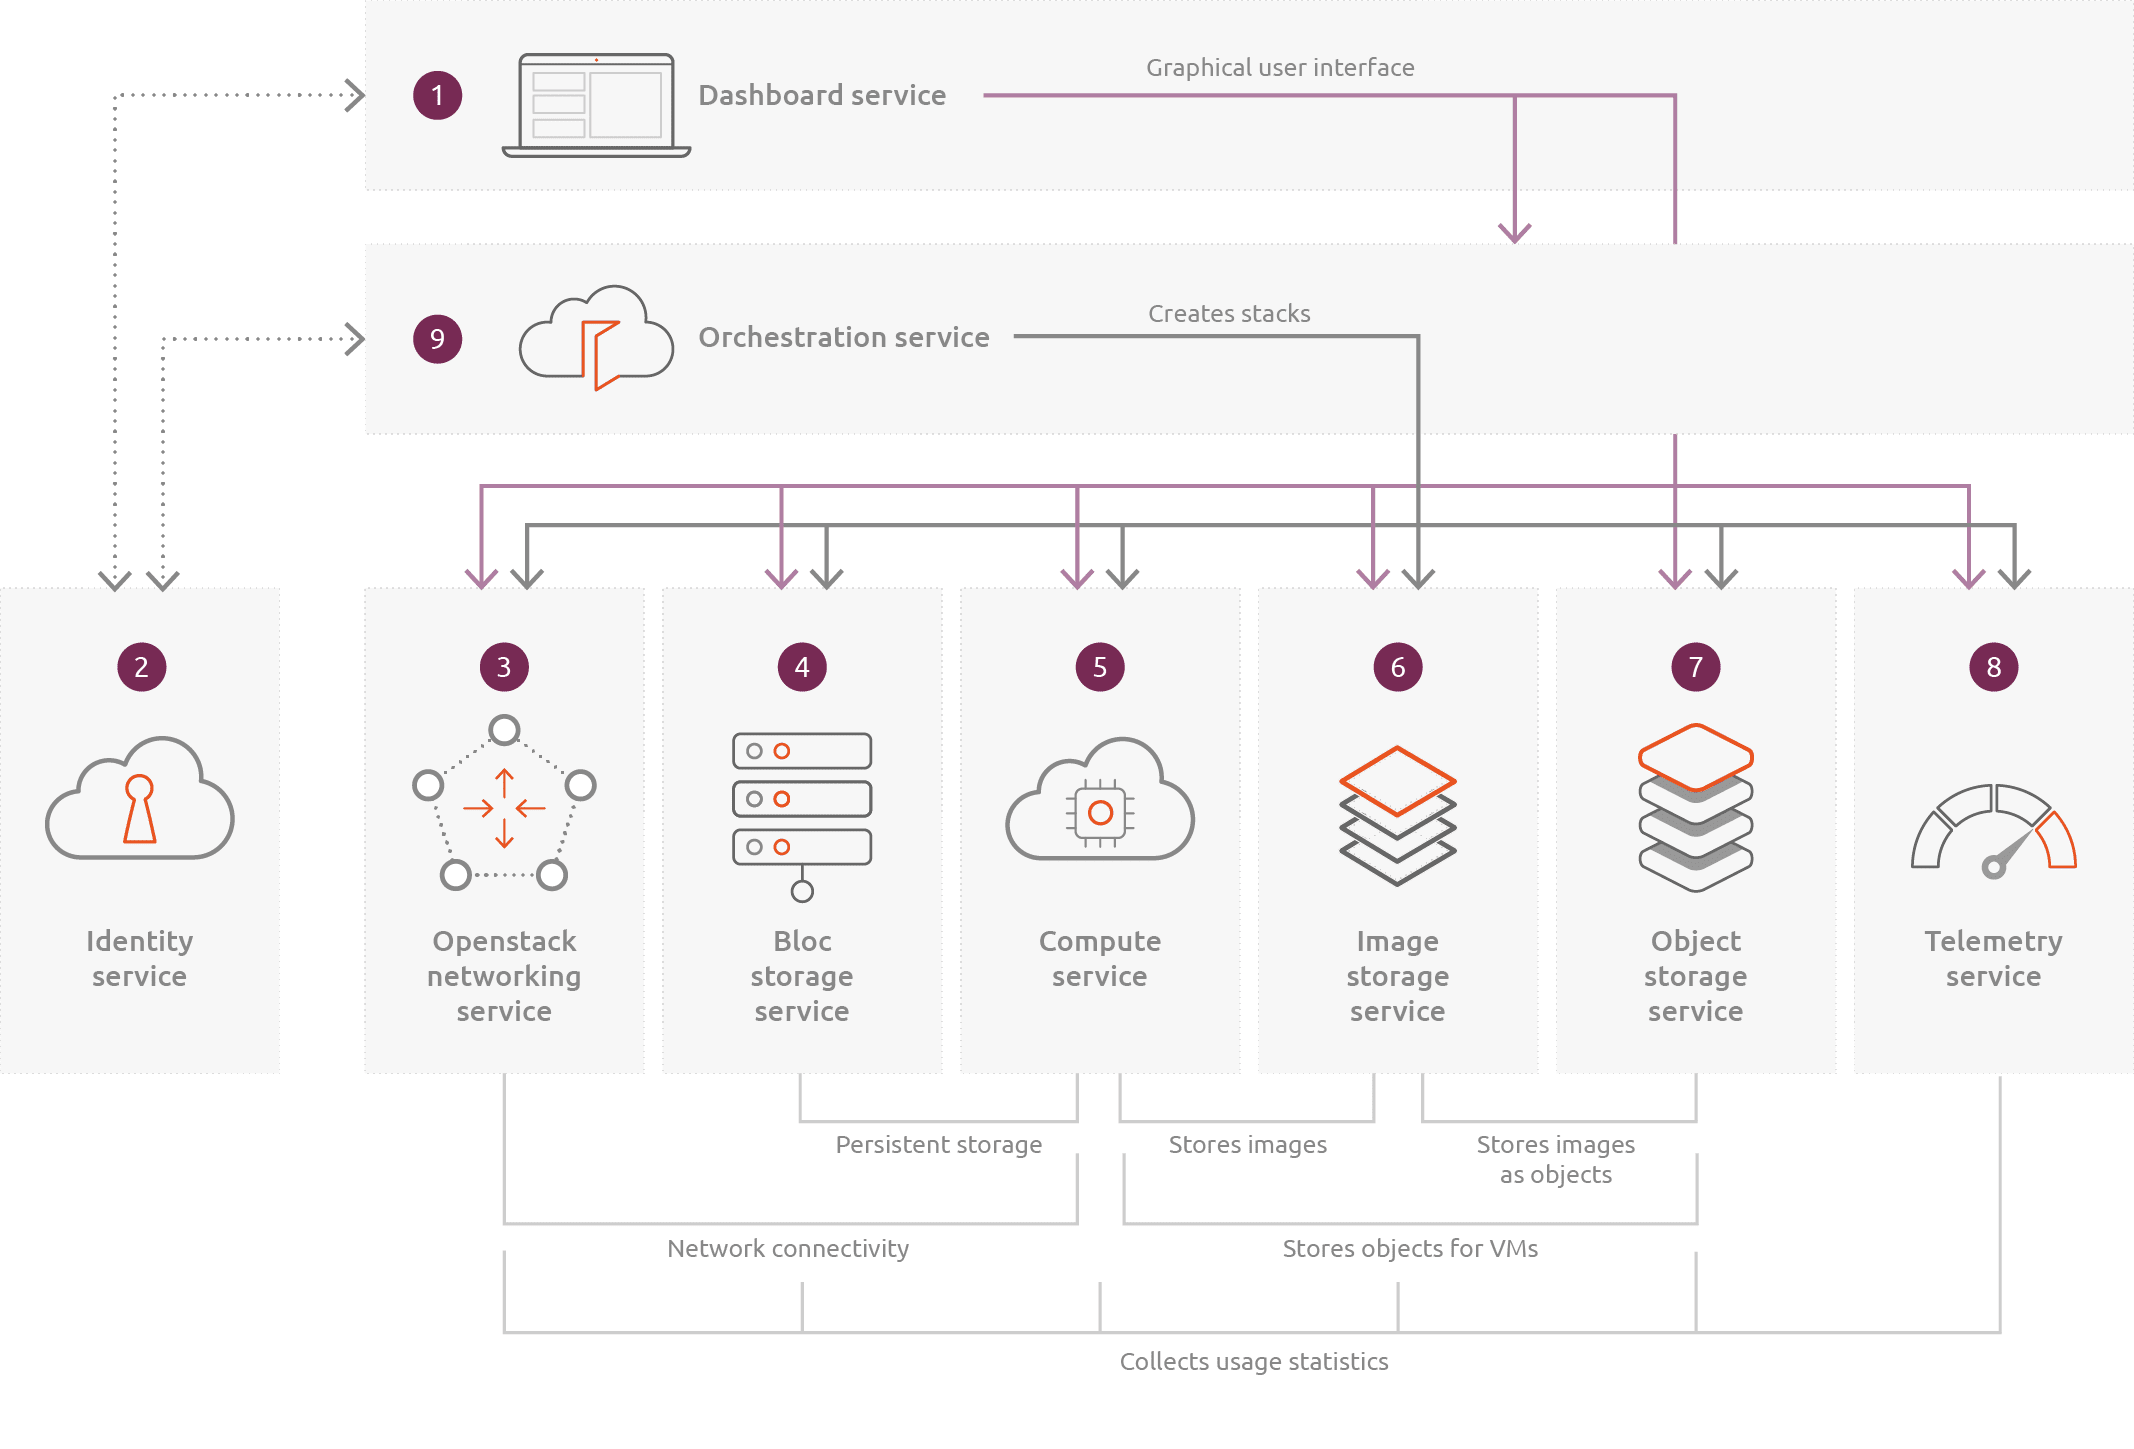
\includegraphics[width=1\textwidth]{images/Openstack.jpg}
\caption{Diagramma rappresentativo funzionamento OpenStack\cite{OpenStack2}}
\end{figure}\\
\subsection{Nova}
\textit{Nova} fa parte del progetto open-source \textit{OpenStack}, e il suo scopo è la gestione delle \textit{Virtual Machine }(\textit{VM}). Esso permette, in simbiosi con Cyborg, di definire gli acceleratori e le FPGA come VM; per maggiori approfondimenti si rimanda a \cite{Nova}.
\subsection{Cyborg}
È un sottosistema di \textit{OpenStack}, il quale si occupa della gestione del ciclo di vita degli acceleratori, il tutto effettuato tramite un'interfaccia \textit{REpresentational State Transfer} (\textit{REST}). Tale approccio permette l'aggiunta e la rimozione di nodi ed informazioni legate ai dispositivi.\cite{Cyborg}
\begin{figure}[h]
\centering
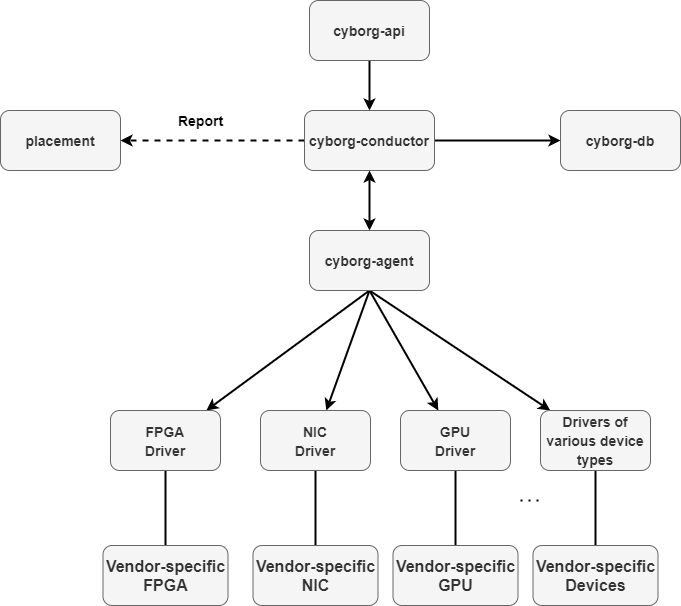
\includegraphics[width=0.7\textwidth]{images/cyborg-architecture.png}
\caption{Architettura del funzionamento di Cyborg\cite{Cyborg}}
\end{figure}\\
Tramite i \textit{driver}, \textit{Cyborg} sarà in grado di interfacciarsi con la scheda FPGA ed effettuare le operazioni discusse approfonditamente nel capitolo \ref{chap:Cap1}
\subsection{Blazar}
\label{Blazar}
È un servizio fornito da \textit{OpenStack} al fine di effettuare la \textit{Resource Reservation}, ossia la prenotazione delle risorsr disponibili nel sistema Cloud. Le prenotazioni possono esser effettuate per un periodo di tempo specifico, immediato o nel futuro; per risorse intendiamo istanze di VM, risorse di storage e risorse puramente computazionali.\cite{Blazar}
\subsection{Iotronic - Lightning-Rod}
Essi sono due servizi che tramite le \textit{REST API}, permettono la gestione di device \textit{IoT} denominati all'interno del framework come "board"; la struttura dei servizi è conforme a quella dei servizi di \textit{OpenStack}, quindi integrabile nel sistema.\\
L'architettura del sistema si concentra sulla comunicazione tra gli user ed i nodi \textit{IoT}. I servizi sono due, e si differenziano dipendentemente dal lato dell'infrastruttura che operano; \textit{IoTronic} lavora lato Cloud, mentre \textit{Lighting-Rod} lato \textit{IoT}; la combinazione dei due permette di realizzare varie azioni volte alla gestione dei dispositivi IoT,
\begin{itemize}
    \item La gestione delle Board, come l'invio dei comandi;
    \item Plugin;
    \item Servizi;
    \item Virtual Network;
    \item Web Service;
\end{itemize}
\textit{Lightning-rod}, come detto, rappresenta il punto di contatto tra il Sistema Operativo, presente sulla Processing System dell'FPGA SoC, ed il Cloud. Permettendo all'utente di interfacciarsi attraverso una comunicazione assicurata tramite WAMP.
